\chapter{LCS Nodes and EasyEda}

The schematics and boards shown were all developed using the EasyED software. EasyEDA is a design tool for developing the schematics and PCB layouts. A PCB can then be ordered at very reasonable prices. Even during LCS node early design stages it is therefore sometimes worthwhile to just produce a PCB and avoid searching software bugs that are actually just loose connection on a breadboard. To ease the development, there are experimental boards. However when it comes to a final design, PCB boards need to be developed and ordered in larger quantitates. The LCS Node design introduced contains a main controller board and extension boards. The sizes and location of the connectors have been standardized. This appendix contains the PCB drawings of the most common LCS boards to give you a head start in developing your own boards, ensuring that all boards fit together.

\section{Symbols and Footprints}

EasyEDA allows you to create symbols that represent components and can be placed in a schematic. To each symbol there should be a footprint that is used to put the component on to the PCB. The connection between the two is a list of assignments that associate a \textbf{pin} on the symbol with a \textbf{pad} on the footprint. For LcsNodes there is a list of symbols and footprints to ensure that the PCBs do have all their connectors at the exact place, so that they fit together.

\subsection{Symbols}

To ease the development of LCS boards, the entire board and its connectors are available as a symbol. Depending on the category, the symbol features the connection end points for the connectors found on the board. This symbol is associated with the corresponding footprint described in the next section. Note that the footprint needs to match the symbol. That is the number, position and meaning of the connectors found on the board map, only length of the PCB board varies.

\subsection{Main Controller Board Footprints}

This section contains all the footprints available so far. There are three main categories. The first is anything that represents an LCS Controller portion. There are the connections to the LCS bus and the power input connector. On the left side are two connectors. The upper connector is reserved for up to four tack pow lines. Below is the LCS extension board connector. The basic LCS Main Controller Board for example is the 16cm x 10cm board shown below.

\begin{figure}[htbp]
    \centering
    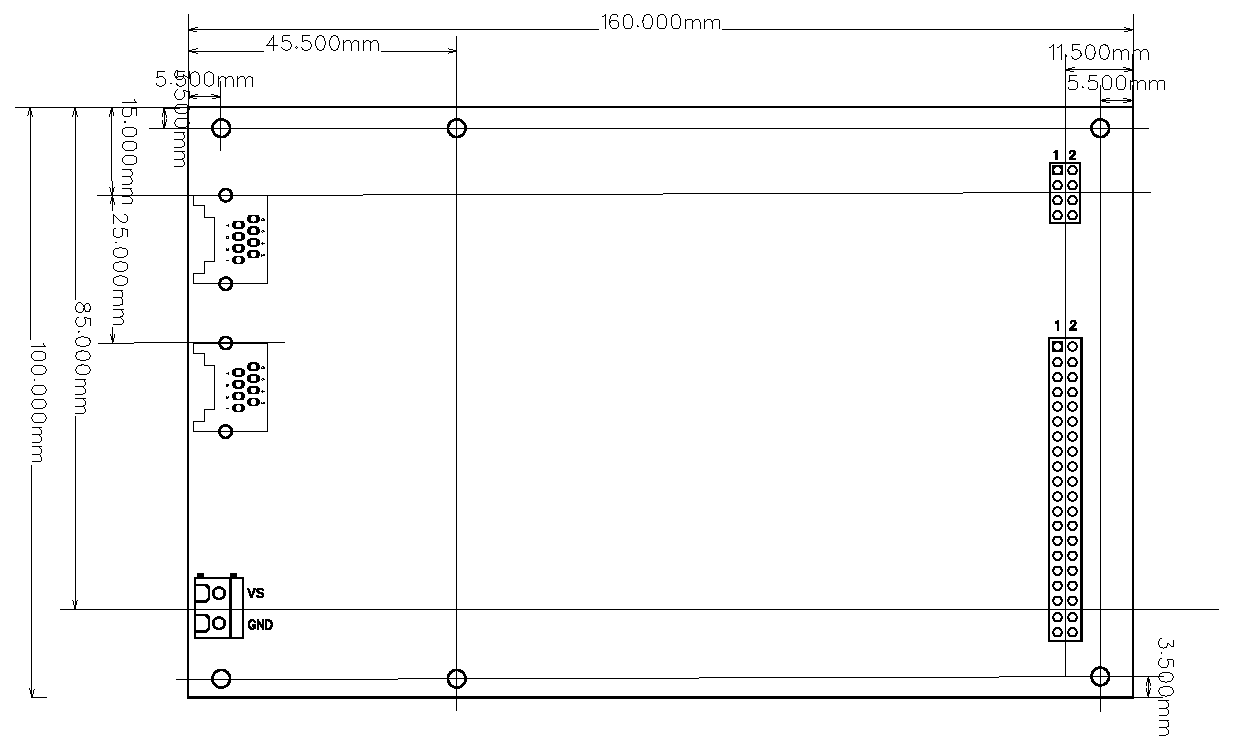
\includegraphics[page=1, scale=0.7]{./Figures/LCS-FP-MAIN-CTRL-10X16.pdf}
    \caption{LCS-FP-MAIN-CTRL-10X16}
    %\label{fig:your-label}
\end{figure}

\FloatBarrier

The mounting holes may look a little odd. As shown in the text to follow, there are extension boards with a form factor of 12cm x 10cm. When are the are mounted on top of the 16cm board, the holes nicely match. 

\section{Extension Boards Footprints}

Next, there are the extension boards. The extension board has the LCS connectors on the left side. The right hand side will typically host the connectors to the layout. These boards can either directly plugged into a controller board or into a bus PCB which hosts controller and more than one extension board. In either case, the extension boards are the same.

\begin{figure}[htbp]
    \centering
    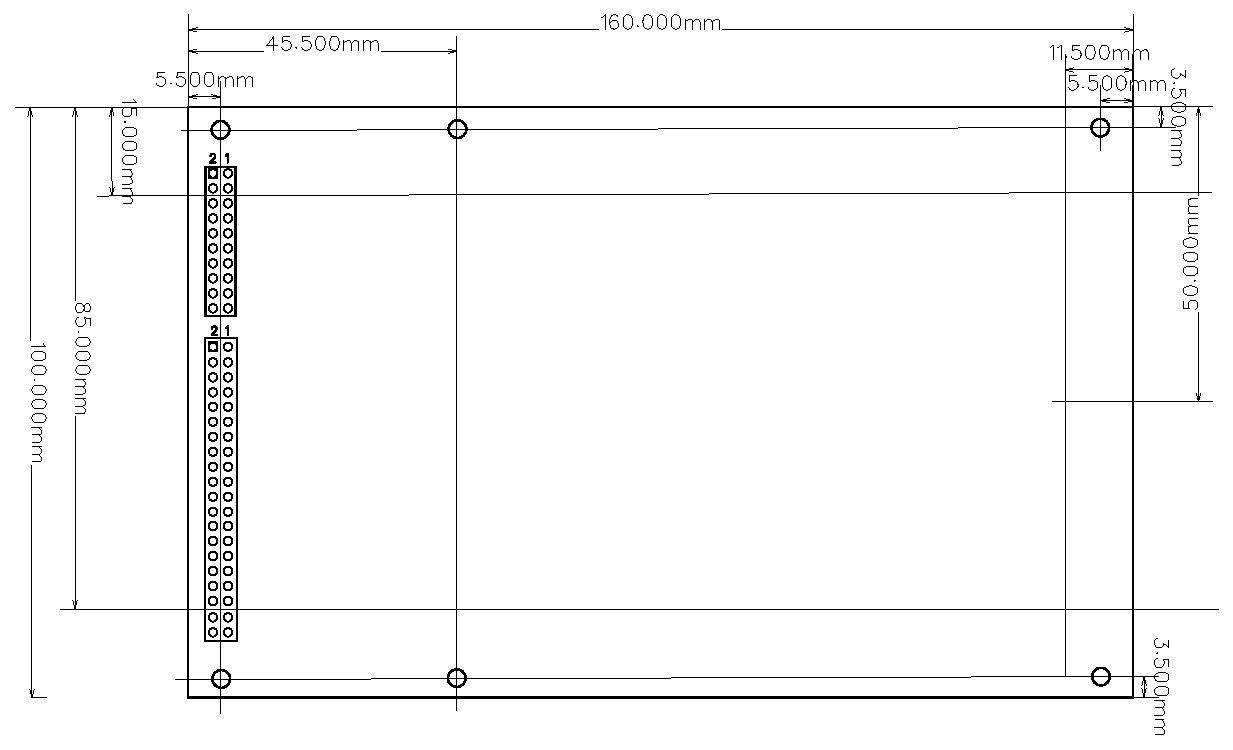
\includegraphics[page=1, scale=0.7]{./Figures/LCS-FP-EXT-L-10X16.pdf}
    \caption{LCS-FP-EXT-R-10X16}
    %\label{fig:your-label}
\end{figure}

\FloatBarrier

In addition to the basic 16cm x 10cm form factor is a set of 12cm x 10cm boards. They have exactly the same layout, except that their length is 12cm instead of 16cm. As always, there could be many more combinations as new boards with different demands are developed. Nevertheless it is important that when connectors are used, that they have the same meaning and are placed at the same location. This is the whole idea of using footprints to ensure this exact fitting.

\section{Pad Numbers}

In EasyEDA, the symbol pads and the PCB pads meet via PAD numbers. Across all symbols and PCBs the numbers assignments are shown in the figure below.

\begin{figure}[htbp]
    \centering
    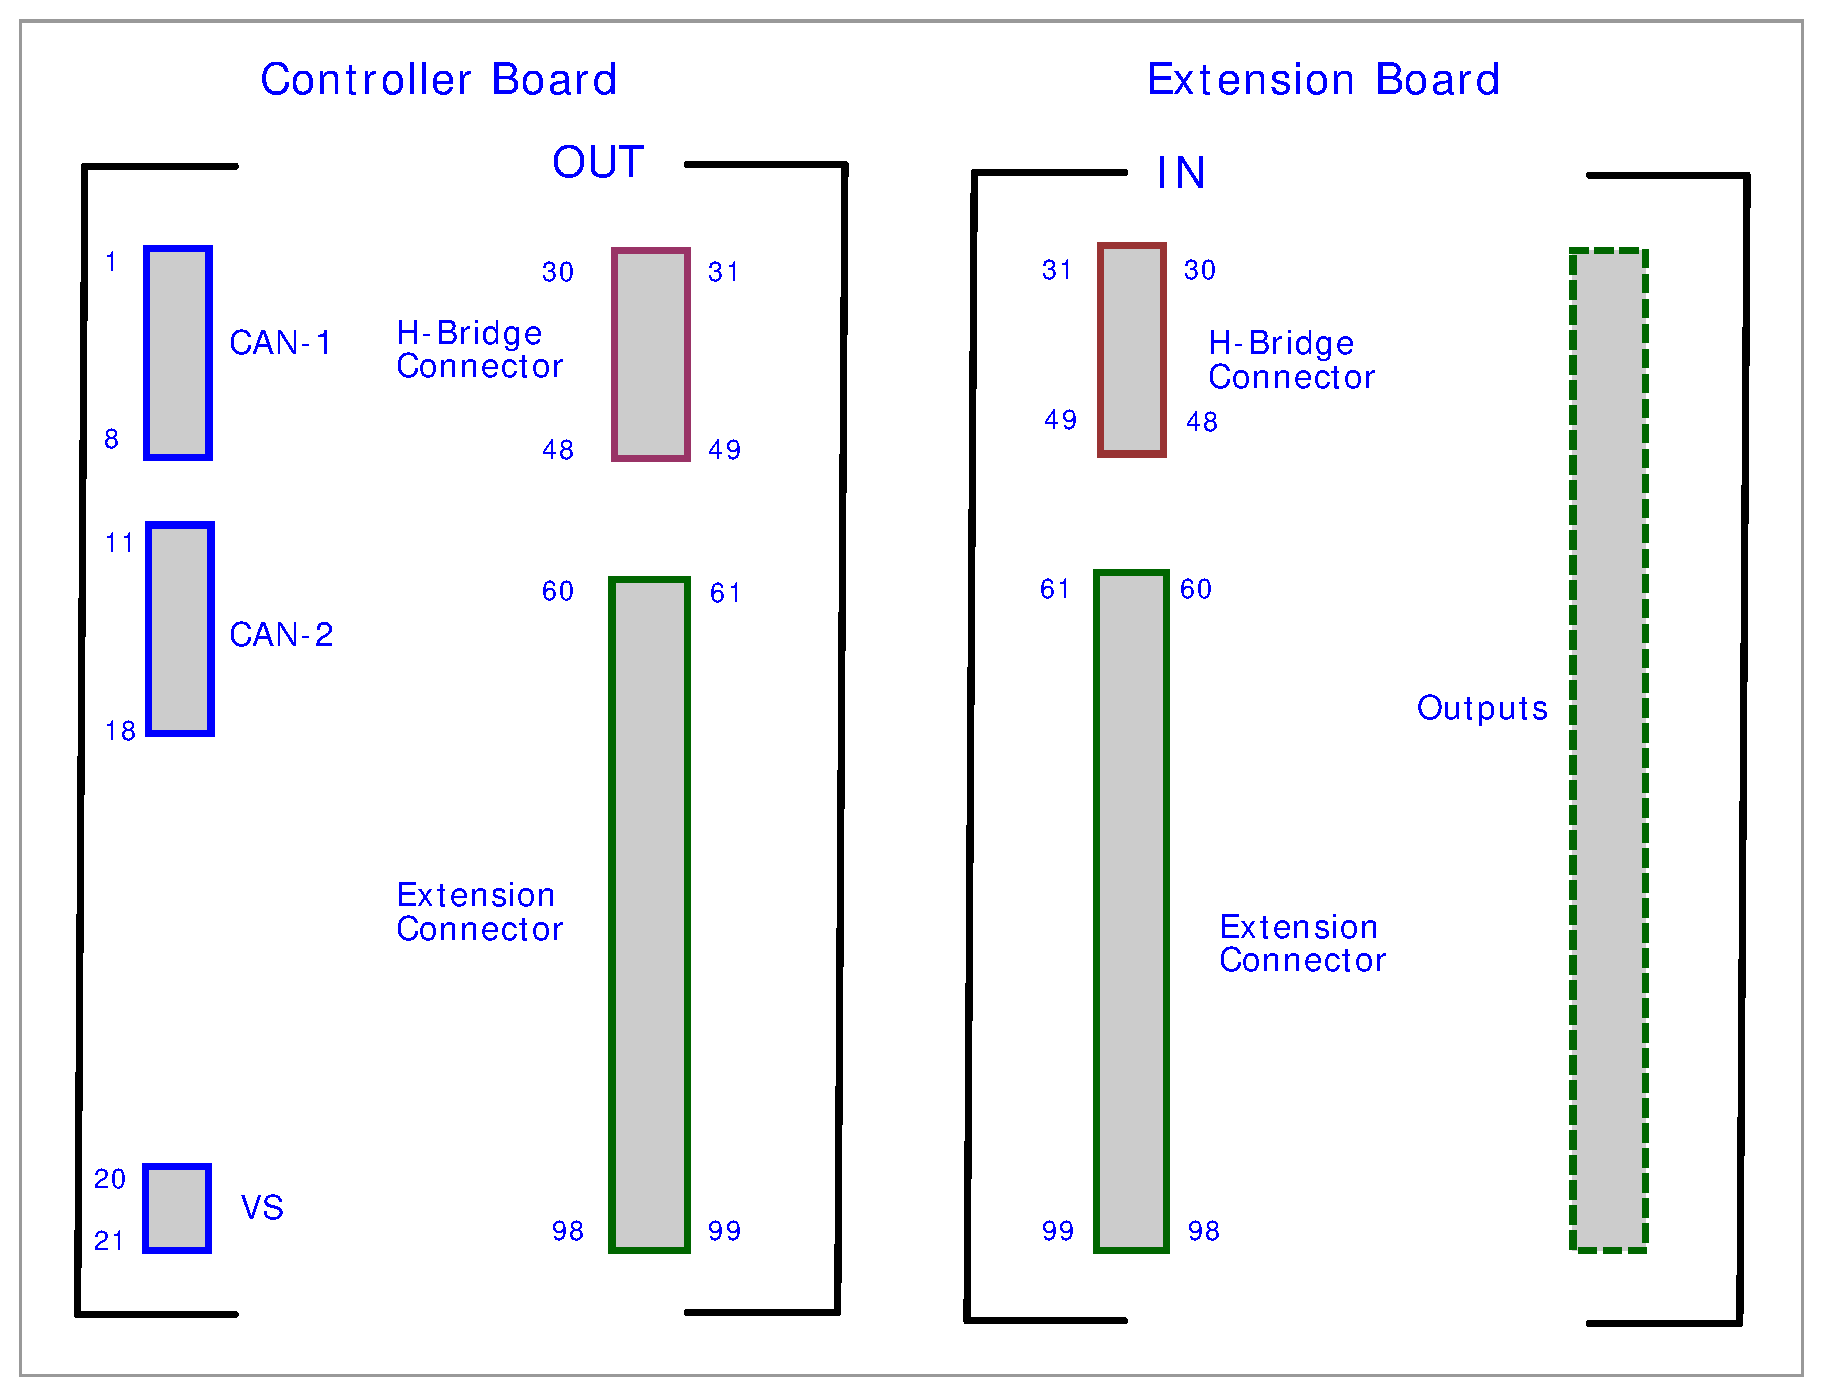
\includegraphics[page=1, scale=0.4]{./Figures/PCB-Connector-Footprint-Pad-Numbers.pdf}
    \caption{PCB-Connector-Footprint-Pad-Numbers}
    %\label{fig:your-label}
\end{figure}

\FloatBarrier

\section{Links}

\begin{table}[!ht]
    \begin{center}
        \caption{...}
        \begin{tabular}{|l|l|p{0.5\textwidth}|}
            \toprule
            \textbf{Tool} & \textbf{Link} & \textbf{Comment} \\
            \midrule
            EasyEDA & http://easyeda.com/de & Design tool for schematics and PCB layouts \\
            \midrule
            JLCPCB & - & PCB board manufactures and parts provider, order from within EasyEDA \\
            \bottomrule
        \end{tabular}
    \end{center}
\end{table}
